\documentclass{article}
\usepackage{graphicx} % Required for inserting images
\usepackage{float}
\usepackage{subcaption}

\title{Gradient Descent}
\author{Phan Thanh Binh}

\begin{document}

\maketitle

\section{Implementation}
\begin{itemize}
\item Firstly, we need 2 functions: f(x) and f\_(x) corresponds the main function to find the minimum value and its derivatives with respect to x.
\item Secondly, we loop forever until the function value f(x) does not have a significant change compare to the last value. We introduce a tolerance value for this purpose, and also there must be a value to store the last value of f(x).
\item Finally, we need a learning rate and an initial value for x. Then x can be update via the formula: $x = x - lr * f\_(x)$.
\end{itemize}
The full implementation in Python is shown in Figure \ref{fig:impl}.
\begin{figure}[H]
    \centering
    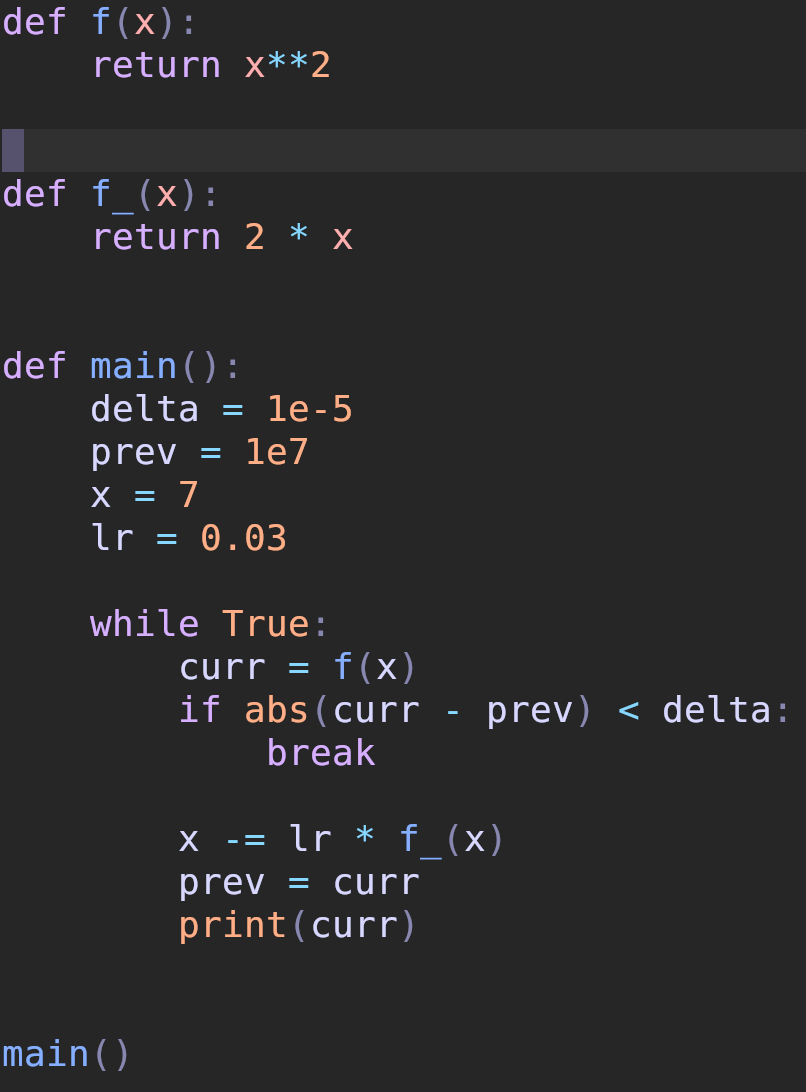
\includegraphics[width=0.5\linewidth]{impl.png}
    \caption{Python Implementation}
    \label{fig:impl}
\end{figure}

\section{Learning rate effect}
We test the code with different learning rate and plot the loss over the first 10 time steps.
The initial value for x is 7.
The effect is clearly shown in the Figure \ref{fig:lrs}, as too big learning rate lead to loss divergence, while too small can lead to slow convergence.
\begin{figure}[H]
\centering
\begin{subfigure}{0.4\textwidth}
    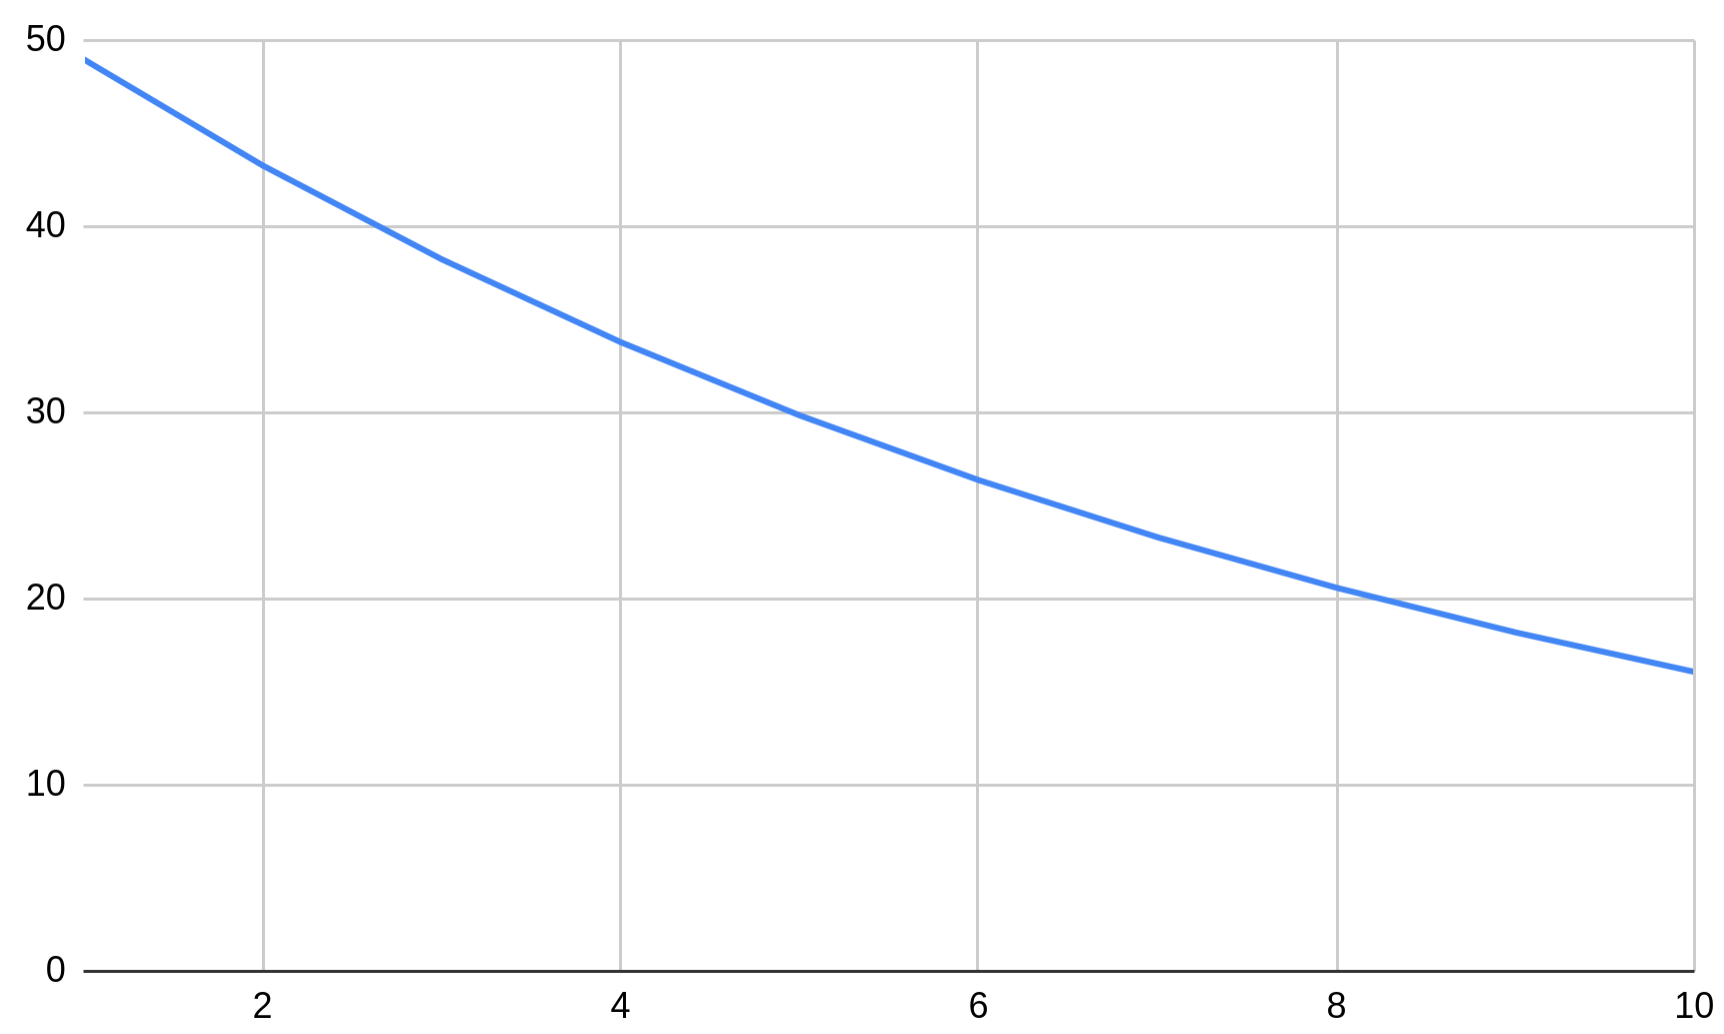
\includegraphics[width=\linewidth]{lr0.03.png}
    \caption{Learning rate = 0.03}
    \label{fig:lr0.03}
\end{subfigure}
\begin{subfigure}{0.4\textwidth}
    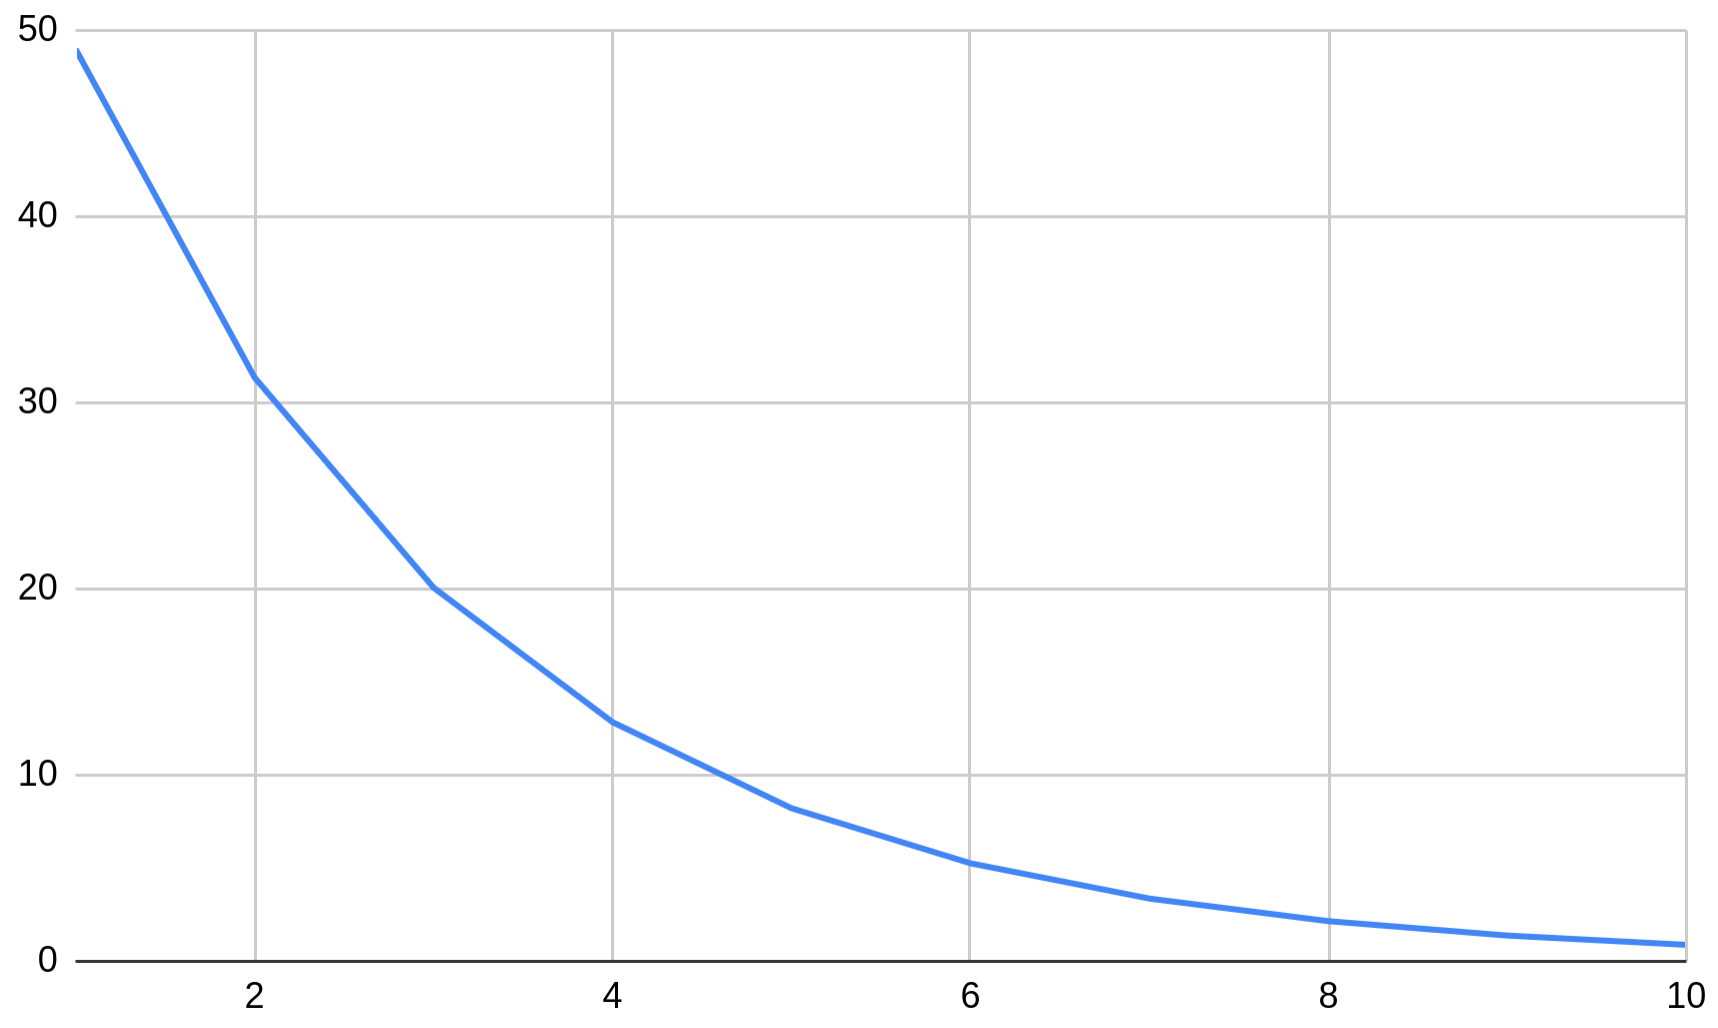
\includegraphics[width=\linewidth]{lr0.1.png}
    \caption{Learning rate = 0.1}
    \label{fig:0.1}
\end{subfigure}
\begin{subfigure}{0.4\textwidth}
    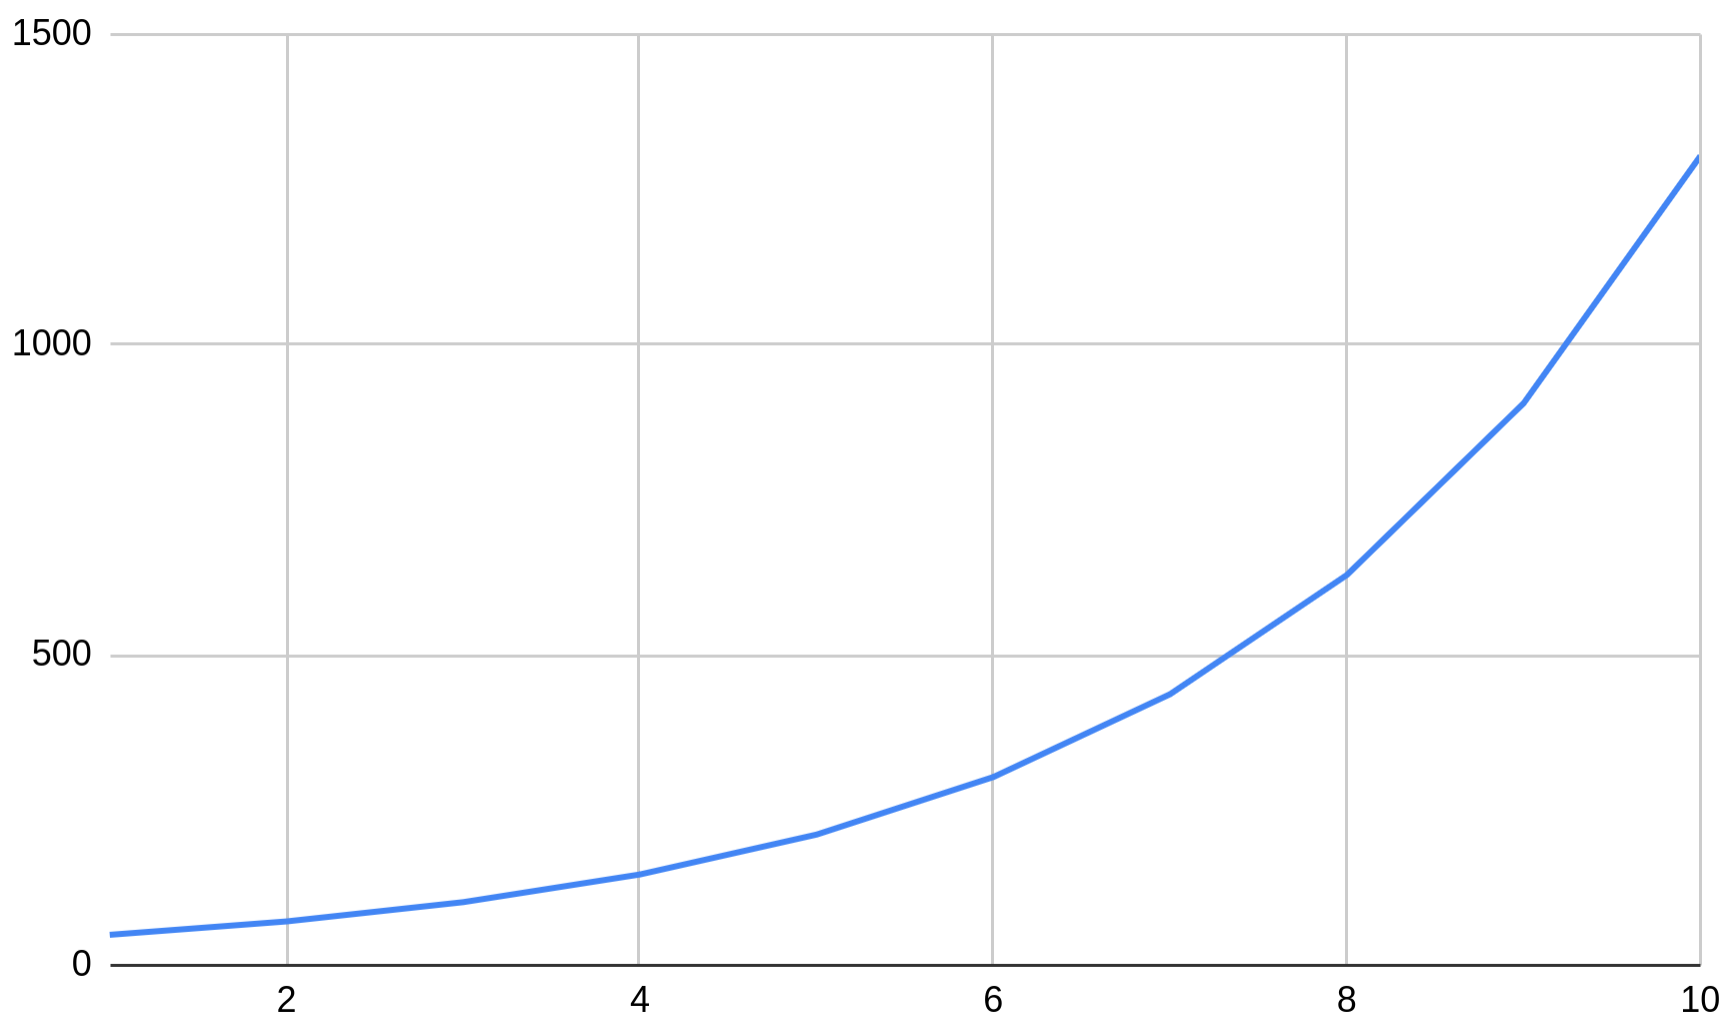
\includegraphics[width=\linewidth]{lr1.1.png}
    \caption{Learning rate = 1.1}
    \label{fig:lr1.1}
\end{subfigure}
\caption{Loss values with first 10 time steps with different learning rate}
\label{fig:lrs}
\end{figure}

\end{document}
